% !TEX encoding = UTF-8 Unicode
\documentclass[a4paper,12pt]{extreport}
\usepackage[utf8]{inputenc}
\usepackage{color}
\usepackage[T2A]{fontenc}
\usepackage[intlimits]{amsmath}
\usepackage{amssymb}
\usepackage{dsfont}
\usepackage{bm}
\usepackage{indentfirst}
% \usepackage[1cm]{fullpage}
\usepackage{geometry}
\usepackage{soul}
\usepackage[normalem]{ulem}
\usepackage[english,russian]{babel}
\usepackage{hyperref}
\hypersetup{
    colorlinks=true,
    linkcolor=blue,
    filecolor=magenta,      
    urlcolor=cyan,
}
\usepackage{mathtools}
\usepackage{graphicx}
\usepackage{multicol}
\usepackage{float}
\graphicspath{{Pictures/}}

% \linespread{1.0}                    % Полуторный интвервал (ГОСТ Р 7.0.11-2011, 5.3.6)
% \Large


% \renewcommand{\labelenumi}{(\alph{enumi})} % Use letters for enumerate
% \DeclareMathOperator{\Sample}{Sample}
\let\vaccent=\v % rename builtin command \v{} to \vaccent{}
\usepackage{enumerate}
\renewcommand{\v}[1]{\ensuremath{\mathbf{#1}}} % for vectors
\newcommand{\gv}[1]{\ensuremath{\mbox{\boldmath$ #1 $}}} 
% for vectors of Greek letters
\newcommand{\uv}[1]{\ensuremath{\mathbf{\hat{#1}}}} % for unit vector
\newcommand{\abs}[1]{\left| #1 \right|} % for absolute value
\newcommand{\avg}[1]{\left< #1 \right>} % for average
\let\underdot=\d % rename builtin command \d{} to \underdot{}
\renewcommand{\d}[2]{\frac{d #1}{d #2}} % for derivatives
\newcommand{\dd}[2]{\frac{d^2 #1}{d #2^2}} % for double derivatives
\newcommand{\pd}[2]{\frac{\partial #1}{\partial #2}} 
% for partial derivatives
\newcommand{\pdd}[2]{\frac{\partial^2 #1}{\partial #2^2}} 
% for double partial derivatives
\newcommand{\pdc}[3]{\left( \frac{\partial #1}{\partial #2}
 \right)_{#3}} % for thermodynamic partial derivatives
\newcommand{\ket}[1]{\left| #1 \right>} % for Dirac bras
\newcommand{\bra}[1]{\left< #1 \right|} % for Dirac kets
\newcommand{\braket}[2]{\left< #1 \vphantom{#2} \right|
 \left. #2 \vphantom{#1} \right>} % for Dirac brackets
\newcommand{\matrixel}[3]{\left< #1 \vphantom{#2#3} \right|
 #2 \left| #3 \vphantom{#1#2} \right>} % for Dirac matrix elements
\newcommand{\grad}[1]{\gv{\nabla} #1} % for gradient
\let\divsymb=\div % rename builtin command \div to \divsymb
\renewcommand{\div}[1]{\gv{\nabla} \cdot \v{#1}} % for divergence
\newcommand{\curl}[1]{\gv{\nabla} \times \v{#1}} % for curl
\let\baraccent=\= % rename builtin command \= to \baraccent
\renewcommand{\=}[1]{\stackrel{#1}{=}} % for putting numbers above =
\providecommand{\wave}[1]{\v{\tilde{#1}}}
\providecommand{\fr}{\frac}
\providecommand{\RR}{\mathbb{R}}
\providecommand{\NN}{\mathbb{N}}
\providecommand{\seq}{\subseteq}
\providecommand{\e}{\varepsilon}

% LaTeX internal stuff
\newcommand{\innermid}{\nonscript\;\delimsize\vert\nonscript\;}
\newcommand{\activatebar}{%
  \begingroup\lccode`\~=`\|
  \lowercase{\endgroup\let~}\innermid 
  \mathcode`|=\string"8000
}

% Probability theory
\newcommand{\Expect}{\mathop{{}\mathrm{E}}}
\newcommand{\Expectmore}{\operatorname{E}\expectarg}
\newcommand{\covmore}{\operatorname{cov}\expectarg}
\DeclarePairedDelimiterX{\expectarg}[1]{[}{]}{%
  \ifnum\currentgrouptype=16 \else\begingroup\fi
  \activatebar#1
  \ifnum\currentgrouptype=16 \else\endgroup\fi
}
\newcommand{\Proba}{\mathrm{P}}
\newcommand{\Var}{\mathop{{}\mathrm{V}}}

% Stochastic processes
\newcommand{\generaltime}{t \geqslant 0}
\newcommand{\discretetime}{t = 1,\,2,\,\ldots}
\newcommand{\conttime}{t \in \realline^{+}}
\newcommand{\finiteconttime}[1]{0 \leqslant t \leqslant #1}
\newcommand{\finitediscretetime}[1]{\running{t}{1}{#1}}

\newcommand{\newprocess}[1]{
	\ensuremath{
		#1 = \left(#1 _t\right)_{\generaltime}
	}
}
\newcommand{\newprocessd}[1]{
	\ensuremath{
		#1 = \left(#1 _t\right)_{\discretetime}
	}
}
\newcommand{\newprocessfc}[2]{
	\ensuremath{
		#1 = \left(#1 _t\right)_{\finiteconttime{#2}}
	}
}

\newcommand{\trajectory}[1]{\big\{#1_s,\,0\leqslant s \leqslant t\big\}}
\newcommand{\firsttime}[1]{\ensuremath{\inf \{\generaltime: #1\}}}

\newcommand{\filtration}[1]{\mathcal{#1}}
\newcommand{\filtrationprocess}[2]{\filtration{#1}^{#2}}
\newcommand{\filtrationflow}[1]{\newprocess{\filtration{F}}}

\newcommand{\fbm}{B^H}

\geometry{paper=a4paper,top=1cm,bottom=2cm,left=1cm,right=1cm}

\begin{document}


% \begin{center}
%     \begin{tabular}{|p{15.5cm}|}
%         \hline
%         \textbf{ФКН ВШЭ, 3 курс, 3 модуль}\\
%         \begin{center} \Large Проверочная работа 2. Авторегрессионные
%         и~условно-гауссовские модели временных рядов
%         \end{center}\\
%         \textbf{Вероятностные модели и статистика случайных процессов, весна 2017}\\
%         \hline
%     \end{tabular}
% \end{center}

% Время выдачи задания: 10 февраля (пятница), 12:10.

% Срок сдачи: \textcolor{blue}{\bf 10 февраля (пятница), 12:40.}

% \section*{Правила сдачи}

% \begin{enumerate}
% \item Работу необходимо сдать преподавателю на листе бумаги
% до дедлайна.
% \item Сверху листа укажите ваши фамилию и имя.
% \item \textbf{Каждая из задач имеет стоимость 1 балл.}
% Максимально допустимая оценка за работу -- 10 баллов. 
% \end{enumerate}


% \section*{Условия задач}


\begin{enumerate}

	\item Опишите свойства временного ряда, изображенного на картинке,
	в терминах
	\begin{enumerate}
		\item наличия тренда,
		\item наличия сезонности,
		\item стационарности 2-го порядка (постоянства моментов),
		\item гомоскедастичности.
	\end{enumerate}

	\begin{figure}[h!]
	\centering
	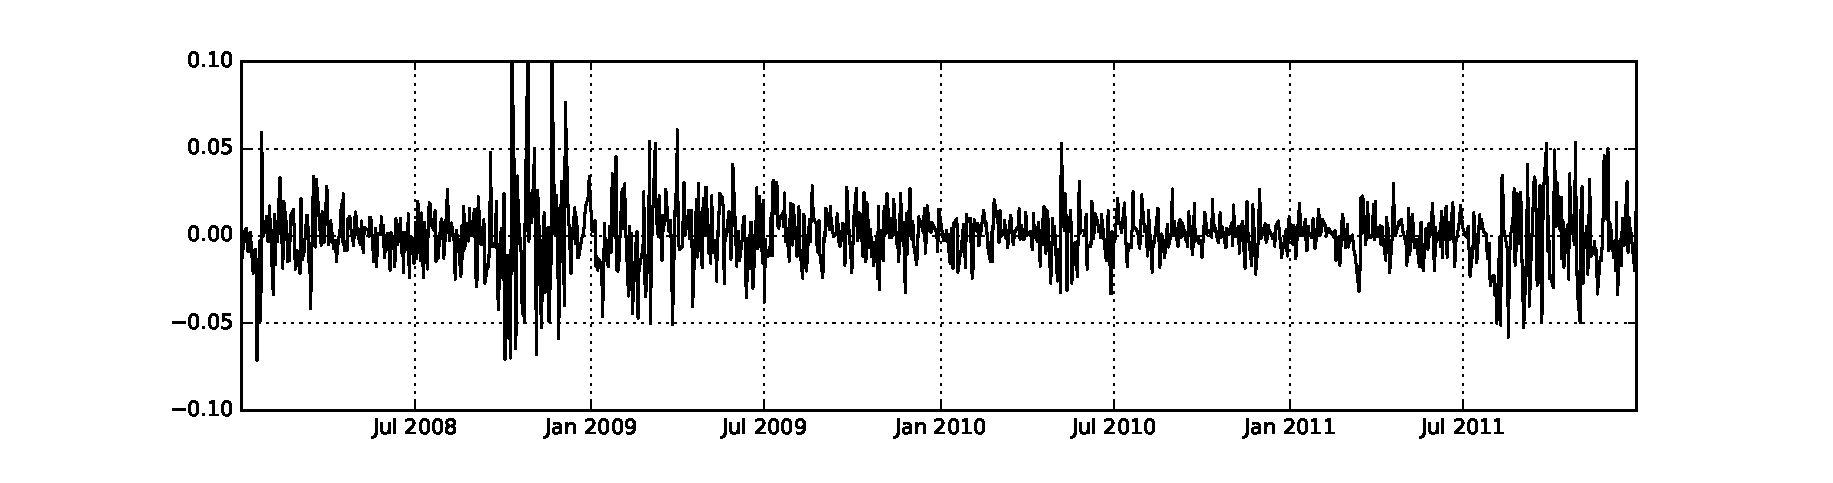
\includegraphics[width=\textwidth,
	trim=1cm 5mm 1cm 5mm, clip=True]
	{dax}
	\end{figure}	

	\item Следующий код на языке \texttt{python} генерирует некоторый случайный процесс:
	\vspace{-.5em}
	\begin{verbatim}
import numpy as np
eps = np.random.normal(size=1000)
series = np.zeros_like(eps)
for i in xrange(len(eps) - 1):
    series[i + 1] = 0.7 * series[i] + eps[i + 1]
	\end{verbatim}
	\vspace{-.5em}
	Объясните, какой случайный процесс моделируется. 
	Запишите описывающие его уравнения.

	\item Рисунок 2 (левый) показывает смоделированные
	траектории трех случайных процессов.

	\begin{figure}[h!]
	\centering
	\begin{minipage}{0.45\textwidth}
	\centering

	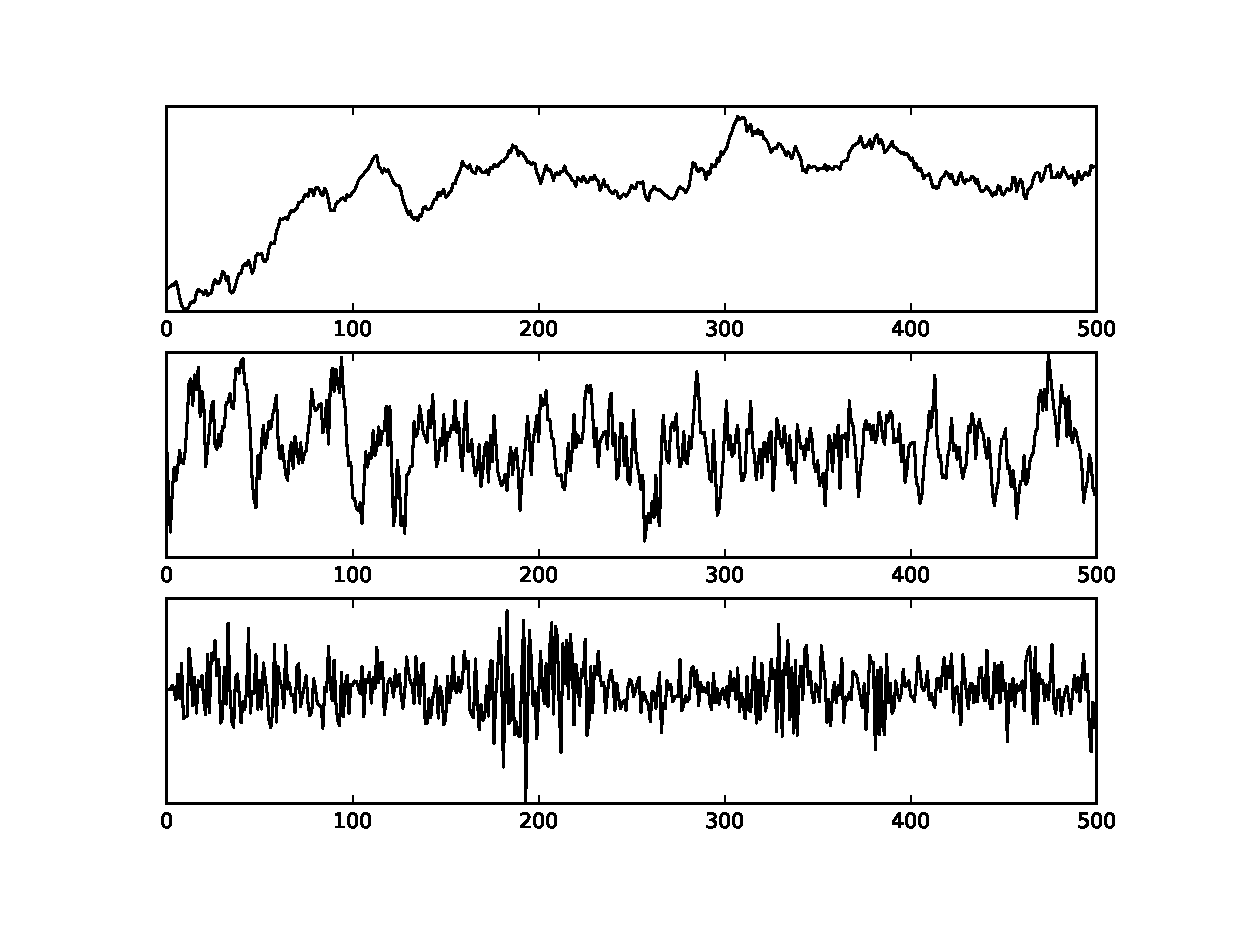
\includegraphics[width=0.9\textwidth,
	trim=1cm 10mm 1cm 10mm, clip=True]
	{bm_ar_arch}

	\end{minipage}\hfill
	\begin{minipage}{0.5\textwidth}
	\centering

	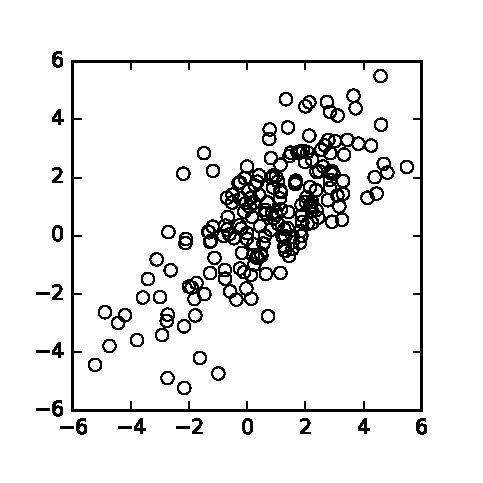
\includegraphics[width=0.5\textwidth,
	trim=2mm 5mm 5mm 5mm, clip=True]
	{xt_xtm2_corr}

	\end{minipage}
	\end{figure}

		Какая из траекторий может относиться к стационарному процессу AR(1)?
	Обоснуйте ваш ответ.

	\item Рисунок 3 (правый) получен по реализации смоделированного
	случайного процесса $\newprocess{X}$, причем каждая точка представляет
	собой пару $(X_{t-2}, X_t)$. Корреляция точек на рисунке равна $0.8$.
	Ответить на вопросы:
	\begin{enumerate}
		\item Какая стохастическая модель могла использоваться для
		моделирования временного ряда? Обоснуйте ответ.
		(Подсказка: искомый процесс принадлежит к одному из типов
		$X_t = \varepsilon_t$; $X_t = \varepsilon_t + \beta \varepsilon_{t-1}$;
		$X_t = c + a X_{t-1} + \varepsilon_t$; $X_t = c + X_{t-1} + \varepsilon_t$;
		$X_t = c - X_{t-1} + \varepsilon_t$.)
		\item Запишите уравнение модели, используя знание типа модели
		и автокорр. функции.
		\item Как можно смоделировать такой процесс на компьютере?
		Напишите соответствующую программу.
	\end{enumerate}

	\item Пусть случайный процесс $\newprocess{X}$ задан своей моделью 
	$X_t = 3 + 0.5 X_{t-1} + \varepsilon_t$, где $\newprocess{\varepsilon}$ -- 
	процесс белого шума, $\Expect \varepsilon_t = 0, \Expect \varepsilon^2_t = 1$.
	\begin{enumerate}
		\item Запишите тип модели процесса $X$.
		\item Объясните, почему модель процесса $X$ является
		<<условно-гауссовской>>, подсчитайте ее условные математическое 
		ожидание и дисперсию. Это модель <<условного математического ожидания>>
		или <<условной дисперсии>>?
		\item Предположим, что дано наблюдение $X_t = 2.5, X_{t-1} = 1.7$. 
		Подсчитайте прогноз значения случайной величины $X_{t+1}$.
		\item Предположим, что дано наблюдение $X_t = 2.5, X_{t-1} = 1.7$. 
		Подсчитайте оценку дисперсии процесса в момент $t+1$ 
		(оценку дисперсии случайной величины $X_{t+1}$).
	\end{enumerate}

	\item Какие из указанных ниже процессов являются слабо стационарными?
	(Процесс $\newprocess{\varepsilon}$ -- белый шум.)
	\begin{enumerate}
		\item $X_t = 1.6 + X_{t-1} + \varepsilon_t$;
		\item $X_t = 0.6 + X_{t-1} + \varepsilon_t$;
		\item $X_t = 0.8 X_{t-1} + \varepsilon_t$;
		\item $X_t = 0.8 \varepsilon_t + 0.6 \varepsilon_{t-1}$;
		\item $X_t = \varepsilon_t \sqrt{2 + 2X^2_{t-1}}$.
	\end{enumerate}

	\item Рассмотрим стохастическую модель 
	$X_t = \varepsilon_t \sqrt{\alpha_0 + \alpha_1 X^2_{t-1}}$,
	где $\newprocess{\varepsilon}$ -- 
	белый шум, $\Expect \varepsilon_t = 0, \Expect \varepsilon^2_t = 1$.
	\begin{enumerate}
		\item Запишите тип модели процесса $X$.
		\item Возможно ли осуществить выбор постоянных
		$\alpha_0$ и $\alpha_1$ таким образом, чтобы эта модель 
		хорошо описывала гетероскедастичный временной ряд? 
		Обоснуйте ваш ответ.
	\end{enumerate}

	\item Доходность акций часто оценивают в процентах согласно следующей формуле.
	Если $S_n$ -- цена закрытия акции в день $n, n \geqslant 1$, то ее доходность равна величине
	$X_n = \frac{S_n - S_{n-1}}{S_n}$ (отношение прироста цены закрытия
	за текущий день к цене предыдущего дня, daily returns in percent). 

	GARCH-модель была подогнана к временному ряду
	дневной доходности акций. Вывод оценивающего алгоритма, предполагающего
	гауссовский белый шум, представлен ниже:
	\vspace{-.5em}
	\begin{verbatim}
    Estimate  Std. Error    t value   Pr(>|t|)
a0  0.027832    0.006282       4.43   9.41e-06 ***
a1  0.009064    0.008813      16.67    < 2e-16 ***
b1  0.830477    0.008813      94.24    < 2e-16 ***
	\end{verbatim}
	\vspace{-.5em}
	Средняя доходность равна 0.0492.
	\begin{enumerate}
		\item Запишите уравнения модели, определяющие процесс доходности акций.
		\item Вычислите долгосрочную дисперсию доходности указанной модели.
		\item Предположим, сегодняшняя доходность равна $+1.5\%$; прогноз
		дисперсии на сегодня равен $\widehat{\sigma}^2_t = 1.1619$. 
		Подсчитайте распределение завтрашней доходности.
		\item Истинная завтрашняя доходность оказалась равной $+4.6\%$. 
		Что можно сказать о найденном в (c) распределении доходности?
	\end{enumerate}
	(Подсказки: $X_t = \sigma_t \varepsilon_t$;
	$\sigma^2_t = \alpha_0 + \alpha_1 \sigma^2_{t-1}$;
	$\Expect X_t = 0$; $\Expectmore{X_t | X_{t-1}} = 0$; 
	$\Expect X^2_t = \frac{\alpha_0}{1 - \alpha_1 - \beta_1}$;
	$\Expectmore{X^2_t | X^2_{t-1}} = \sigma^2_{t-1}$.)

% 	\item Следующий код на языке \texttt{python} моделирует GARCH процесс:
% 	\begin{verbatim}
% N = 1000
% nu = np.random.normal(size=N + 50)
% eps = np.zeros(N + 50)
% h = np.zeros(N + 50)
% a0 = 1
% a1 = 0.1
% a2 = 0.07
% b1 = 0.82
% for i in xrange(2, N + 50):
%     h[i] = a0 + a1 * eps[i-1]**2 + a2*eps[i-2]**2 + b1*h[i-1]
%     eps[i] = nu[i]*np.sqrt(h[i])
% # eps = eps[-1:50]
% 	\end{verbatim}

% 	\begin{enumerate}
% 		\item Запишите порядок процесса.
% 		\item Подгоните GARCH модель к траектории. Проверьте,
% 		коррелирован ли временной ряд квадратов отклонений.
% 		\item Подгоните модель GARCH(1, 1) (неверную!) к траектории. Проверьте,
% 		коррелирован ли временной ряд квадратов отклонений. Видно ли, что модель
% 		задана неправильно?
% 		\item Увеличьте $N$ до 10000 и снова выполните (c).
% 		(Мощность теста гипотезы $H_0$ о том, что во временном ряде
% 		отсутствует автокорреляция, возрастает с ростом длины ряда.)
% 	\end{enumerate}

% 	\item 



\end{enumerate}


\end{document}
